\documentclass[11pt]{article}


  \usepackage[review]{acl}

\usepackage{times}
\usepackage{latexsym}
\usepackage[T1]{fontenc}
\usepackage[utf8]{inputenc}
\usepackage{microtype}
\usepackage{booktabs}
\usepackage{amsmath}
\usepackage{amssymb}
\usepackage{graphicx}
\usepackage{url}


\graphicspath{{figures/}}

\title{Chunking in RAG:\\
A Controlled Audit and Multi-Dataset Robustness Study}

  \author{Anonymous Authors}

\date{}
\makeatletter
\setlength{\@fptop}{0pt}
\setlength{\@dblfptop}{0pt}
\makeatother
\begin{document}
\maketitle

\begin{abstract}
We revisit document chunking in retrieval-augmented question answering through two
complementary studies. First, we audit an archived Mistral-7B pilot on 60 SQuAD~2.0
and 30 HotpotQA questions. Although recursive-256 has the highest observed F1, no
post-hoc contrast is significant after Holm correction. Replaying the exact prompts
shows that the 1,024-token generator limit truncates every SQuAD fixed-512 prompt and
that MiniLM truncates 93.9\% of the corresponding corpus chunks during embedding. A
corrected failure audit also attributes 59.1\% of recursive HotpotQA exact-match
failures to incomplete retrieval rather than repairable generation.
Second, a prospective robustness extension varies three data seeds, three retriever
families, two embedding models, and four encoder-compatible chunkers over larger
SQuAD and HotpotQA samples and a new technical-support domain, TechQA. The best
observed chunker changes across datasets, embedders, and retrievers; for example,
switching from MiniLM to BGE raises the best dense HotpotQA AllHit@4 from
$50.7\pm4.8$ to $70.2\pm8.9$. Controlled local Qwen2.5-1.5B and Mistral-7B studies
also select dataset-specific observed winners. None of 18 recursive-versus-comparator
contrasts survives a single Holm correction across both generators and all three
datasets. These results reject a universal chunker ranking and show why token budgets
and system components must be reported together.
\end{abstract}

\section{Introduction}

Retrieval-augmented generation (RAG) conditions a language model on external evidence
rather than relying exclusively on parametric memory \citep{lewis2020rag}. Most RAG
systems index chunks instead of complete documents. A chunking policy therefore affects
the retrieval unit, the amount of surrounding context, the number of indexed vectors,
and the evidence that can fit into the generator prompt. These effects are coupled: a
larger chunk may preserve discourse while exceeding an encoder or prompt budget, whereas
a smaller chunk may fit easily but omit neighboring evidence.

We use a two-stage design. The first stage is a retrospective audit of an archived
Mistral experiment in which the sampled corpus, embedding model, dense retriever,
retrieval depth, prompt, generator, and evaluation code were fixed. The second is a
prospectively specified extension that varies datasets, data seeds, retriever families,
embedding models, and the generator while keeping each within-cell comparison paired.
Together, the studies ask:
\begin{enumerate}
  \item How do six chunker configurations compare on answer quality and
        supporting-document retrieval in the archived pipeline?
  \item How uncertain are the observed paired differences on the sampled questions?
  \item Do encoder and generator token limits change what each nominal chunking
        configuration actually exposes to the system?
  \item Do observed chunker rankings persist across larger samples, a technical-support
        dataset, dense and lexical retrieval, two embedding models, and two controlled
        local generators?
\end{enumerate}

This paper makes four contributions. First, it provides a controlled archival pilot
with per-question predictions and separate answer and evidence-retrieval metrics.
Second, it adds paired bootstrap intervals, randomization tests, and an overlap analysis
showing that identical aggregate recall can conceal different missed questions. Third,
it reconstructs the exact retrieved contexts and replays both tokenizer budgets. This
audit changes the interpretation of the original experiment: some differences are
inseparable from embedding and prompt truncation, and an earlier claim that most
failures were ``fixable'' is not supported. Fourth, it executes a larger robustness
extension across three datasets, three seeds, three retriever families, two embedding
models, and controlled local generation with Qwen2.5-1.5B and Mistral-7B. The extension
directly tests---and does not support---a dataset- or architecture-independent chunker
ranking.

Code, configurations, per-question predictions, and audit outputs are included in the
anonymous supplementary material.

\section{Related Work}

\paragraph{RAG and dense retrieval.}
RAG combines retrieval with conditional generation \citep{lewis2020rag}; Dense Passage
Retrieval established bi-encoder retrieval as a strong approach for open-domain QA
\citep{karpukhin2020dpr}. Our implementation follows this broad design but does not use a
DPR checkpoint: it embeds chunks with all-MiniLM-L6-v2, a Sentence-BERT-style
encoder \citep{reimers2019sentencebert} derived from MiniLM
\citep{wang2020minilm}, and searches normalized embeddings with inner product. The
robustness extension also uses BGE-small-en-v1.5, an English embedding checkpoint from
the BGE/FlagEmbedding family \citep{xiao2023cpack}, and compares dense retrieval with
BM25 and weighted reciprocal-rank fusion.

\paragraph{Segmentation and retrieval granularity.}
Topical text segmentation predates neural retrieval; TextTiling, for example, detects
subtopic boundaries from lexical cohesion \citep{hearst1997texttiling}. Recent work
treats retrieval granularity as an empirical variable. Dense X Retrieval shows that the
choice of retrieval unit affects both retrieval and downstream QA
\citep{chen2024densex}. Semantic chunking attempts to align boundaries with embedding
similarity, but its cost-benefit trade-off is inconsistent across evaluated settings
\citep{qu2024semanticchunking}. Late Chunking instead contextualizes token embeddings
before pooling, illustrating that segmentation also interacts with when contextual
representations are formed \citep{gunther2024latechunking}. Our study compares boundary
rules within one conventional pre-chunking pipeline; it does not compare these broader
embedding architectures.

\paragraph{RAG and QA evaluation.}
Knowledge-intensive evaluation should distinguish answer correctness from provenance
and evidence retrieval \citep{petroni2021kilt}. Frameworks such as RAGAs and ARES
separate context relevance, answer relevance, and faithfulness
\citep{es2024ragas,saadfalcon2024ares}, while RAGTruth demonstrates that retrieval does
not by itself prevent unsupported generation \citep{niu2024ragtruth}. Reading
comprehension systems are also sensitive to distractors \citep{jia2017adversarial}.
These findings motivate our separate answer, supporting-document, and context-visibility
measurements.

\paragraph{Domains and generators.}
SQuAD and HotpotQA cover Wikipedia reading comprehension and multi-hop reasoning,
respectively \citep{rajpurkar2018squad2,yang2018hotpotqa}. TechQA instead contains
real technical-support questions grounded in product documentation
\citep{castelli2020techqa}. We use NVIDIA's reduced RAG-oriented distribution of that
dataset \citep{nvidia2025techqarag} to test domain transfer. The prospective generation
extension uses pinned local Qwen2.5-1.5B-Instruct \citep{qwen2025qwen25} and
Mistral-7B-Instruct-v0.3 \citep{jiang2023mistral} checkpoints under the same retrieval,
prompt, and decoding protocol. This controlled follow-up is distinct from the archived
Mistral endpoint, whose runtime revision and full server flags were not retained.

\paragraph{Uncertainty and context use.}
Small NLP evaluations require paired tests and explicit uncertainty
\citep{dror2018significance}. Long input capacity is likewise not equivalent to robust
context use: answer accuracy can depend on evidence position even within the nominal
window \citep{liu2024lost}. Our audit addresses an earlier-stage issue---whether the
retrieved evidence enters the model input at all---by replaying the exact truncation
policy before interpreting retrieval-generation discrepancies.

\section{Experimental Setup}

\subsection{Study Structure}

We distinguish the \textit{archival pilot} from the \textit{prospective extension}
throughout. The pilot is a single seed-42 Mistral run reconstructed from stored
predictions; its audits cannot retroactively recover missing raw drafts or endpoint
metadata. The extension was executed after the audit with pinned dataset and model
revisions, retained raw generations and prompt-length traces, and configurations chosen
to remove the pilot's most severe encoder-budget mismatch. Results from the extension
test robustness rather than replacing or pooling with the archival measurements.

\subsection{Datasets and Corpus Construction}

\paragraph{SQuAD 2.0.}
We use only answerable validation questions \citep{rajpurkar2018squad2}. After a
seed-42 shuffle, the loader takes a 500-example candidate pool and selects 60 questions
round-robin across titles. Context paragraphs sharing a selected title are concatenated,
yielding 35 article-level pseudo-documents. This title-balanced procedure is not a simple
random sample of SQuAD~2.0, and none of SQuAD's unanswerable questions is evaluated.

\paragraph{HotpotQA.}
We select 30 seed-42 validation examples from the distractor configuration
\citep{yang2018hotpotqa}. Each question has two supporting titles and ten candidate
documents. The retrieval corpus is the union of the question-level candidates: 300
documents. This construction differs materially from the 35-document SQuAD corpus.

\paragraph{TechQA.}
The extension adds NVIDIA TechQA-RAG-Eval, a reduced RAG-oriented distribution of IBM
TechQA \citep{castelli2020techqa,nvidia2025techqarag}. It contains real
technical-support questions, long product-support documents, and complete explanatory
answers rather than mostly short Wikipedia spans. We filter out rows marked impossible
or lacking contexts and sample evaluation questions after a seeded shuffle. Retrieval
always searches the same closed corpus of 496 unique context documents from all
answerable rows, rather than a question-conditioned set of gold documents. A filename
identifies a gold support document.

\paragraph{Extension sample sizes.}
For retrieval-only evaluation, each of seeds 13, 21, and 34 selects 150 SQuAD questions
from a 900-example candidate pool, 75 HotpotQA distractor questions, and 200 answerable
TechQA questions. SQuAD retains the title-round-robin procedure; HotpotQA and TechQA use
seeded shuffled samples. Both prospective generator runs use seed 42 and the same 60,
30, and 50 questions from SQuAD, HotpotQA, and TechQA, respectively. Thus the retrieval
extension covers 425 questions per seed, while generation remains a smaller controlled
two-checkpoint study.

\subsection{Chunking Configurations}

Chunk sizes are measured with the MiniLM tokenizer. We compare six configurations from
four families:
\begin{itemize}
  \item \textbf{Fixed windows:} targets of 128, 256, and 512 tokens with overlaps of
        19, 38, and 76 tokens, respectively.
  \item \textbf{Recursive:} a 256-token target and 38-token overlap, using the ordered
        separators paragraph, newline, sentence-ending space, space, and character.
  \item \textbf{Sentence:} a blank English spaCy sentencizer greedily packs complete
        sentences to a 256-token target, without overlap.
  \item \textbf{Semantic:} adjacent sentences are split when MiniLM cosine similarity
        falls below 0.72 after a default 128-token minimum; a 256-token maximum forces a
        split. No overlap is used.
\end{itemize}
Because the algorithms and overlaps differ, the realized chunk-length distributions and
chunk counts are part of each configuration. We therefore compare configurations, not a
single isolated boundary variable.

\paragraph{Prospective extension.}
To fit MiniLM's 256-position encoder budget including two special tokens, the extension
compares four configurations: fixed-128 (19-token overlap), fixed-254 (38-token
overlap), recursive-254 (38-token overlap), and sentence-254 (no overlap). Sentence
segments longer than the target are further split into token-bounded windows. Because
WordPiece decode and re-encode are not always idempotent, every decoded window is
rechecked and shortened until it contains at most 254 content tokens. An executable
audit confirms zero target or encoder-limit violations in every extension cell. We omit
fixed-512 and semantic-256: the former is known to exceed the archival encoder budget,
whereas retaining semantic chunking would introduce an additional encoder-dependent
boundary model into the MiniLM--BGE comparison. These choices narrow the extension to
fixed, separator-aware, and sentence-aware boundaries under a common encoder budget.

\subsection{Embedding and Retrieval}

Chunks are encoded with all-MiniLM-L6-v2; embeddings are L2-normalized and
indexed with FAISS inner-product search. The top four chunks are ranked for every
question. MiniLM's SentenceTransformer configuration has a maximum sequence length of
256 encoded positions, including special tokens. The pipeline raises the separate
tokenizer limit used to create chunks, but not the encoder limit, so overlong chunks are
silently prefix-truncated during embedding. Section~\ref{sec:context-audit} quantifies
this mismatch.

We report \textbf{DocCov@4}, the mean fraction of gold supporting documents represented
among the four retrieved chunks, and \textbf{AllHit@4}, the fraction of questions for
which all supporting documents are represented. These metrics coincide on SQuAD but not
on HotpotQA. We also report \textbf{AnsVis@4}, whether the normalized reference-answer
token sequence occurs inside at least one retrieved chunk. Normalized tokens must match
on token boundaries, preventing short answers such as ``IT'' from matching inside words
such as ``internet.'' HotpotQA yes/no questions are excluded because literal label
presence is not an evidence diagnostic. AnsVis is still conservative for paraphrased and
long TechQA answers, but prevents a hit on an unrelated part of a long gold document from
being mistaken for visible answer evidence.
We omit the repository's original ``Precision@4'' from the main analysis
because it mixes document identity with answer-string containment and counts multiple
chunks from the same document separately.

\paragraph{Prospective retrieval extension.}
We cross the four extension chunkers with dense retrieval, BM25, and hybrid retrieval at
$k=4$. Dense retrieval uses either all-MiniLM-L6-v2 or BGE-small-en-v1.5; the BGE query
is prefixed with its recommended English retrieval instruction
\citep{xiao2023cpack}. The hybrid retrieves 20 candidates from each component and
applies weighted reciprocal-rank fusion with weights 0.6 dense and 0.4 BM25. Since BM25
does not use the embedding model and both configurations use the same pinned MiniLM
chunk tokenizer, its exactly matching result is shared rather than interpreted as two
independent encoder runs. For each dataset--retriever--embedder--chunker cell, we report
mean AllHit@4 and the sample standard deviation across the three data seeds.

\subsection{Prompt, Generator, and Stored Output}
\label{sec:generation}

The generator is the Mistral 7B Instruct v0.3 checkpoint \citep{jiang2023mistral},
served through an OpenAI-compatible vLLM endpoint. The first completion uses temperature 0,
at most 48 new tokens, and a complete-chat input limit of 1,024 Mistral tokens. The
system message instructs the model to use only the context, copy the shortest supported
answer span, omit explanations, and return exactly \textit{unanswerable} when support is
insufficient. HotpotQA passages include titles; SQuAD passages do not. Appendix
\ref{app:prompts} gives the exact messages.

If the formatted chat is too long, the implementation binary-searches for the longest
prefix of the concatenated, rank-ordered context that keeps the complete chat at or below
1,024 tokens. It can remove later chunks or cut inside one. A first-line normalizer then
strips answer labels and citations. Sentence-like or long drafts may trigger a second
Mistral refinement call with at most 24 new tokens, followed by question-dependent
compression rules. Consequently, the archived predictions are stored post-processed
answers, not raw model generations. The artifact does not retain which examples invoked
refinement or the intermediate draft; if refinement returns an empty string or
\textit{unanswerable}, the implementation retains the first draft.

The no-context comparator uses a different short-answer system prompt. It is therefore a
useful descriptive comparator, not a formal lower bound on the contextual system.

\paragraph{Controlled local generator extension.}
The prospective generation study runs pinned Qwen2.5-1.5B-Instruct
\citep{qwen2025qwen25} and Mistral-7B-Instruct-v0.3 \citep{jiang2023mistral} checkpoints
with BGE-small-en-v1.5, the same 0.6/0.4 hybrid retriever, the same retrieved chunk IDs,
and the four extension chunkers. Mistral is loaded locally in float16 rather than through
a paid or mutable hosted endpoint. Each model uses its native chat template and tokenizer,
but receives the same instructions. Greedy decoding permits at most 96 new tokens within
a 1,536-token complete-chat budget for SQuAD and HotpotQA; TechQA permits 512 new tokens
because its references are substantially longer. SQuAD and HotpotQA use the archival
extractive instruction; TechQA uses a concise-but-complete grounded-answer instruction
because its references are often multi-sentence support resolutions. The implementation
stores raw and normalized predictions, full and retained prompt lengths, generated-token
counts, and truncation and length-stop indicators. It preserves multiline TechQA answers
and does not invoke the archival endpoint's refinement call. Each model also has a
no-context run with a different instruction; these are descriptive comparators, not formal
lower bounds.

\subsection{Answer Metrics and Statistical Analysis}

We use SQuAD-style Exact Match (EM) and token F1: lowercase, remove punctuation and
articles, normalize whitespace, and take the maximum over gold references. F1 is the
primary answer endpoint. The repository's marginal intervals resample questions; this
revision uses 20,000 draws for the reported percentile intervals. We additionally align
systems by example ID, bootstrap paired F1 differences with 20,000 draws, and run
two-sided paired sign-flip tests with 100,000 draws. The five post-hoc comparisons of
\texttt{recursive\_256} to the other chunkers are Holm-corrected within each dataset.
All random procedures use seed 8677.

For each prospective generator, we apply the same 20,000-draw paired bootstrap and
100,000-draw sign-flip procedure to F1, comparing recursive-254 with the other three
chunkers. The primary Holm family contains all 18 post-hoc tests across two generators,
three datasets, and three comparators; within-dataset values are retained only for
transparency. Marginal table intervals use 2,000 question-bootstrap draws. Retrieval-only
means use three data seeds and are reported with sample standard deviations; with only
three seeds, we avoid treating their dispersion as a precise population confidence
interval.

The archival intervals express variation over sampled questions conditional on one
recorded run; the prospective intervals are likewise conditional on one deterministic
run per checkpoint. They do not capture generator-run or software variation.
Question-level resampling also
ignores dependence among SQuAD questions from the same title and may be optimistic. The
three-seed retrieval summary directly measures data-sample variation but does not
represent model or deployment variation.

\subsection{Context-Budget and Failure Audits}

We deterministically reconstruct the seed-42 corpora and all six chunk sets, map each
archived retrieved chunk ID back to its text, and replay the Mistral chat template and
prefix-truncation algorithm. Reconstructed chunk counts match the stored counts for every
cell. For each question we record the full prompt length, retained context fraction,
number of completely retained chunks, support-document coverage among those complete
chunks, and whether a normalized SQuAD gold answer remains in the consumed context.

For predictions with EM$=0$, we use three coarse diagnostic categories. A SQuAD case is
\textit{evidence-limited} when no normalized gold answer survives in the reconstructed
post-truncation context. A HotpotQA case is evidence-limited unless both supporting
documents occur among completely retained chunks. Among the remainder, refusals and
strict token-set containment mismatches are \textit{response-form candidates}; other
high-, partial-, and zero-overlap outputs are \textit{answer-content mismatches}. The
priority order is fixed and mutually exclusive. These automatic labels generate
hypotheses; they are neither human causal judgments nor proof that a prompt or
post-processor will repair a prediction.

\section{Results}

\subsection{Observed QA and Retrieval Results}

% Generated by scripts/generate_revision_tables.py; do not edit by hand.

\begin{table*}[t]
\centering
\small
\setlength{\tabcolsep}{4.1pt}
\begin{tabular}{lrrrrrrr}
\toprule
System & EM & F1 & F1 95\% CI & DocCov@4 & AllHit@4 & Avg. tokens & \# chunks \\
\midrule
No context & 13.3 & 29.2 & [20.9, 38.1] & -- & -- & -- & -- \\
\texttt{fixed\_128} & 38.3 & 50.7 & [39.9, 61.4] & \textbf{95.0} & \textbf{95.0} & 125.3 & 631 \\
\texttt{fixed\_256} & 38.3 & 56.7 & [46.2, 66.9] & 88.3 & 88.3 & 244.0 & 322 \\
\texttt{fixed\_512} & 40.0 & 53.7 & [43.1, 64.5] & 90.0 & 90.0 & 472.2 & 164 \\
\texttt{recursive\_256} & \textbf{41.7} & \textbf{60.6} & [50.5, 70.5] & 91.7 & 91.7 & 175.8 & 389 \\
\texttt{sentence\_256} & 35.0 & 51.0 & [40.2, 61.7] & 86.7 & 86.7 & 223.9 & 302 \\
\texttt{semantic\_256} & \textbf{41.7} & 56.9 & [46.1, 67.3] & \textbf{95.0} & \textbf{95.0} & 144.8 & 467 \\
\bottomrule
\end{tabular}
\caption{Observed results on the fixed SQuAD 2.0 sample. EM, F1, DocCov@4, and AllHit@4 are percentage points. Intervals are question-level percentile-bootstrap intervals and do not measure run-to-run variation. Bold marks the largest observed chunker mean; it does not indicate statistical significance.}
\label{tab:squad-results}
\end{table*}

% Generated by scripts/generate_revision_tables.py; do not edit by hand.

\begin{table*}[t]
\centering
\small
\setlength{\tabcolsep}{4.1pt}
\begin{tabular}{lrrrrrrr}
\toprule
System & EM & F1 & F1 95\% CI & DocCov@4 & AllHit@4 & Avg. tokens & \# chunks \\
\midrule
No context & 10.0 & 27.7 & [16.2, 40.0] & -- & -- & -- & -- \\
\texttt{fixed\_128} & 20.0 & 36.5 & [22.7, 51.2] & 75.0 & 50.0 & 89.3 & 421 \\
\texttt{fixed\_256} & 20.0 & 34.3 & [19.8, 49.8] & 75.0 & 50.0 & 114.2 & 313 \\
\texttt{fixed\_512} & 20.0 & 35.7 & [21.5, 50.8] & \textbf{76.7} & \textbf{53.3} & 117.4 & 301 \\
\texttt{recursive\_256} & \textbf{26.7} & \textbf{42.6} & [26.8, 58.7] & \textbf{76.7} & \textbf{53.3} & 113.6 & 313 \\
\texttt{sentence\_256} & 23.3 & 37.0 & [21.6, 53.0] & \textbf{76.7} & \textbf{53.3} & 112.7 & 313 \\
\texttt{semantic\_256} & 23.3 & 42.4 & [27.6, 57.5] & \textbf{76.7} & \textbf{53.3} & 97.2 & 363 \\
\bottomrule
\end{tabular}
\caption{Observed results on the fixed HotpotQA sample. EM, F1, DocCov@4, and AllHit@4 are percentage points. Intervals are question-level percentile-bootstrap intervals and do not measure run-to-run variation. Bold marks the largest observed chunker mean; it does not indicate statistical significance.}
\label{tab:hotpot-results}
\end{table*}


On the fixed SQuAD sample, \texttt{recursive\_256} has the highest observed F1
(60.6) and ties \texttt{semantic\_256} on EM (41.7). On HotpotQA, recursive and
semantic are nearly tied in F1 (42.6 versus 42.4). These are descriptive rankings:
the F1 intervals are broad, especially for HotpotQA, where recursive spans
26.8--58.7.

DocCov@4 and AllHit@4 expose different aspects of multi-hop retrieval. Recursive
HotpotQA DocCov@4 is 76.7, but both supporting documents are recovered for only
53.3\% of questions. Four chunkers share both aggregate values while their observed F1
ranges from 35.7 to 42.6; aggregate document coverage alone does not resolve which
questions or evidence spans differ.

\subsection{Paired Uncertainty and Retrieval Identity}

% Generated by scripts/generate_revision_tables.py; do not edit by hand.

\begin{table*}[t]
\centering
\small
\begin{tabular}{lrrrr}
\toprule
Comparator & \multicolumn{2}{c}{SQuAD 2.0} & \multicolumn{2}{c}{HotpotQA} \\
\cmidrule(lr){2-3}\cmidrule(lr){4-5}
 & $\Delta$F1 [95\% CI] & Holm $p$ & $\Delta$F1 [95\% CI] & Holm $p$ \\
\midrule
\texttt{fixed\_128} & +9.9 [+2.1, +18.4] & 0.088 & +6.1 [-2.3, +16.3] & 0.809 \\
\texttt{fixed\_256} & +3.9 [-2.9, +11.1] & 0.581 & +8.3 [+0.2, +17.9] & 0.627 \\
\texttt{fixed\_512} & +6.9 [+0.2, +14.4] & 0.190 & +6.8 [-2.0, +16.8] & 0.809 \\
\texttt{sentence\_256} & +9.7 [+2.3, +17.8] & 0.088 & +5.6 [+0.0, +14.4] & 0.998 \\
\texttt{semantic\_256} & +3.7 [-3.2, +11.0] & 0.581 & +0.2 [-6.5, +8.5] & 1.000 \\
\bottomrule
\end{tabular}
\caption{Paired comparisons defined as \texttt{recursive\_256} minus each comparator. We resample aligned questions 20,000 times and compute two-sided paired sign-flip tests with 100,000 draws; $p$-values are Holm-adjusted across the five post-hoc contrasts within each dataset.}
\label{tab:paired-differences}
\end{table*}


No recursive-versus-competitor F1 comparison has Holm-adjusted $p<.05$. The largest
SQuAD observed differences are relative to fixed-128 and sentence-256, but both adjusted
$p$-values are .088. Recursive exceeds semantic by only 3.7 F1 points on SQuAD
(95\% paired CI $[-3.2,11.0]$) and 0.2 on HotpotQA ($[-6.5,8.5]$). The experiment
therefore does not statistically resolve a winning chunker.

Equal aggregate retrieval can also conceal distinct failures. Fixed-128 and semantic-256
each retrieve the SQuAD gold article for 57 of 60 questions. Table~\ref{tab:hit-overlap}
shows that only one miss is shared: each system uniquely covers two questions missed by
the other.

\begin{table}[t]
\centering
\small
\begin{tabular}{lrr}
\toprule
 & \multicolumn{2}{c}{Semantic-256} \\
\cmidrule(lr){2-3}
Fixed-128 & Hit & Miss \\
\midrule
Hit  & 55 & 2 \\
Miss &  2 & 1 \\
\bottomrule
\end{tabular}
\caption{Per-question SQuAD gold-article retrieval overlap. Both systems have
95.0\% DocCov@4, but their three misses are not the same.}
\label{tab:hit-overlap}
\end{table}

\subsection{The Nominal Top Four Often Do Not Reach the Generator}
\label{sec:context-audit}

\begin{figure*}[t]
  \centering
  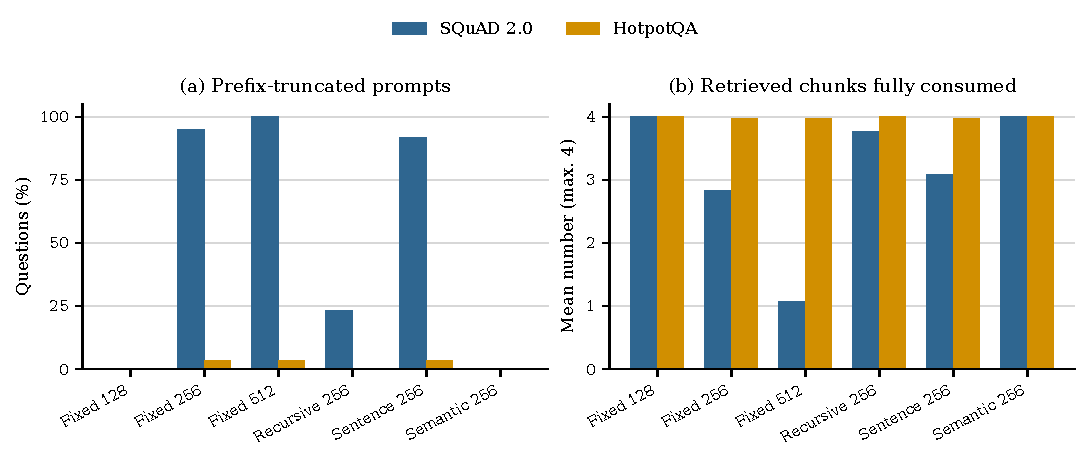
\includegraphics[width=\textwidth]{fig_context_budget.pdf}
  \caption{Replayed 1,024-token context budget. On SQuAD, fixed-256, fixed-512,
  and sentence-256 usually exceed the generator budget; HotpotQA documents are shorter.
  A chunk counted as fully consumed must survive the prefix truncation in its entirety.}
  \label{fig:context-budget}
\end{figure*}

The reviewer's concern about four 512-token chunks and a 1,024-token input is correct.
All 60 SQuAD fixed-512 chats are truncated. Their full prompts average 2,362 Mistral
tokens; after truncation, only 1.07 of four retrieved chunks are completely retained on
average. Fifty-six questions retain chunk~1 plus part of chunk~2, and four retain the
first two plus part of chunk~3; none retains all four. Fixed-256 and sentence-256 are
also truncated for 95.0\% and 91.7\% of SQuAD questions. By contrast, fixed-128 and
semantic-256 are never truncated. Recursive-256 is truncated for 14 of 60 questions,
each retaining three complete chunks and part of the fourth.

The HotpotQA corpus contains much shorter documents: only one fixed-512 question is
truncated, and recursive and semantic prompts are never truncated. The cross-dataset
difference therefore reflects corpus construction as well as nominal chunk size.

The embedding stage introduces a second budget mismatch. MiniLM input length includes
special tokens, leaving at most 254 content wordpieces. This truncates 284 of 322
SQuAD fixed-256 corpus chunks (88.2\%) but only 7 of 389 recursive-256 chunks (1.8\%),
so even the nominally size-matched comparison changes encoder exposure. It also truncates
154 of 164 SQuAD fixed-512 chunks (93.9\%); only 12 of 301 HotpotQA fixed-512 chunks
(4.0\%) are affected. The SQuAD fixed-window results consequently combine boundary
policies with encoder-side and generator-side truncation; they cannot identify a
``large chunk'' mechanism in isolation. Appendix Table~\ref{tab:context-audit} reports
all configurations.

\subsection{Corrected Failure Audit}

% Generated by scripts/generate_revision_tables.py; do not edit by hand.

\begin{table}[t]
\centering
\scriptsize
\setlength{\tabcolsep}{2.2pt}
\begin{tabular}{lrr}
\toprule
Category & SQuAD & HotpotQA \\
\midrule
Evidence limited & 8 (22.9; 12.1--39.0) & 13 (59.1; 38.7--76.7) \\
Form/refusal & 19 (54.3; 38.2--69.5) & 6 (27.3; 13.2--48.2) \\
Content mismatch & 8 (22.9; 12.1--39.0) & 3 (13.6; 4.7--33.3) \\
\bottomrule
\end{tabular}
\caption{Corrected audit of \texttt{recursive\_256} errors (EM$=0$). Cells show count (percentage; Wilson 95\% CI). SQuAD evidence is checked after prompt truncation; HotpotQA requires both supporting documents. Form/refusal labels are hypotheses, not verified fixes.}
\label{tab:failure-audit}
\end{table}


The corrected audit reverses the original HotpotQA interpretation. Among 22 recursive
predictions with EM$=0$, 13 retrieve only one of two supporting documents and are
evidence-limited. Six are response-form candidates after complete document retrieval,
and three are residual answer-content mismatches. Thus the earlier claim that 16 of 22
(72.7\%) were fixable format or refusal errors was produced by treating any nonzero
support coverage as retrieval success. The stricter response-form share is 27.3\%
(Wilson 95\% CI 13.2--48.2), and even this is not a repair rate.

For SQuAD, 8 of 35 recursive EM failures lack a normalized gold answer in the retained
context, 19 are response-form candidates, and 8 are answer-content mismatches. Of four
refusals that retrieve the gold article, only three retain a normalized answer string.
This distinction matters because article-level retrieval does not guarantee that an
answer-bearing span reaches the generator.

\subsection{Prospective Multi-Setting Retrieval Extension}

The retrieval extension does not reproduce one stable ranking. With MiniLM dense
retrieval, the best observed AllHit@4 configuration is fixed-128 on SQuAD
($97.1\pm1.4$), sentence-254 on HotpotQA ($50.7\pm4.8$), and fixed-128 on TechQA
($88.0\pm3.0$). With BGE dense retrieval, the corresponding choices are fixed-128
($97.8\pm0.4$), recursive-254 tied with sentence-254 ($70.2\pm8.9$), and fixed-254
($88.8\pm0.8$). The 19.5-point increase in best dense HotpotQA AllHit@4 from MiniLM to
BGE is larger than the within-encoder gaps among chunkers, illustrating that an
embedding change can dominate the chunking comparison.

Hybrid retrieval changes the picture again. Fixed-128 is best observed on SQuAD for
both MiniLM ($98.9\pm0.4$) and BGE ($99.1\pm1.0$), whereas HotpotQA favors fixed-254
with MiniLM ($48.0\pm5.8$) and recursive-254 with BGE ($58.7\pm3.5$). On the fixed
496-document TechQA corpus, MiniLM hybrid ties fixed-128 and sentence-254 at
$88.7$ AllHit, while BGE hybrid favors fixed-128 ($90.8\pm1.3$). BM25 is
embedding-independent and is reported once conceptually even though the paired
configuration files reproduce it.

Document identity and answer visibility select different chunkers. Sentence-254 has the
highest observed AnsVis@4 in every dense and hybrid cell: for example, on TechQA it
reaches $48.3\pm5.3$ with MiniLM dense and $49.2\pm5.0$ with BGE hybrid, far below the
corresponding best document AllHit values. A gold-document hit therefore often retrieves
the wrong region of a long support document. These are means and sample standard
deviations over three seeds, not significance claims; the extension supports interaction,
not a new universal winner. Table~\ref{tab:robustness-retrieval} reports every dense and
hybrid setting in the appendix.

\subsection{Controlled Local Generation Extension}

Qwen yields dataset-dependent observed rankings. Its highest observed F1 is fixed-128 on
SQuAD (66.58), sentence-254 on HotpotQA (53.37), and fixed-254 on TechQA (23.72).
The no-context F1 values are 17.26, 21.91, and 13.97, respectively, so every observed
RAG mean exceeds its descriptive no-context comparator while absolute TechQA overlap
remains low. Because TechQA references are long resolutions, token F1 measures lexical
coverage but does not establish factual completeness.

No Qwen recursive-versus-comparator contrast is significant: after the primary Holm
correction, all nine Qwen adjusted $p$-values are 1.0. No SQuAD or HotpotQA prompt is
truncated. Across the four TechQA RAG cells, fixed-254 truncates context for 2 of 50
questions and recursive-254 and sentence-254 for 1 each; fixed-128 truncates none. No
Qwen output reaches its configured generation cap.

Mistral also yields dataset-dependent rankings. Fixed-128 has the highest observed
SQuAD F1 (61.59), sentence-254 the highest HotpotQA F1 (49.64), and fixed-254 the
highest TechQA F1 (26.50), compared with no-context F1 values of 27.78, 23.36, and
16.04. Its smallest raw paired value is for recursive-254 minus fixed-128 on SQuAD
($-7.23$ F1, 95\% CI $[-13.62,-1.77]$, raw $p=.0156$), but the global Holm-adjusted
value is $.2817$. None of the 18 planned contrasts across both generators survives the
primary correction. Mistral truncates no SQuAD or HotpotQA prompt and five TechQA RAG
prompts; no output reaches its configured generation cap. The complete two-model matrix,
including marginal intervals, appears in Table~\ref{tab:robustness-generation}.

\section{Discussion}

Across both studies, rankings are conditional on realized encoder and generator budgets,
the retrieval stack, dataset, and generator. Document AllHit and answer visibility can
select different chunkers, while equal aggregate coverage can hide different missed
questions. Chunking recommendations should therefore identify the complete system and
evidence endpoint, and preserve the text actually consumed after truncation.

The extension improves coverage with a new domain, larger multi-seed retrieval samples,
two embedders, three retriever families, and two controlled local generators. It does not
turn response-form diagnostics into proof of repairability: that claim requires a frozen
prompt intervention evaluated on held-out questions. Appendix~\ref{sec:additional-discussion}
states the prospective protocol and remaining interpretive cautions.

\section{Conclusion}

The evidence does not support a portable best chunk size. The pilot is confounded by
encoder and prompt truncation, and its corrected HotpotQA audit finds incomplete
retrieval more often than repairable generation. In the extension, observed winners
change across datasets and system components, and no post-hoc contrast survives the
18-test correction. Future chunking studies should match token budgets, retain consumed
evidence and raw outputs, sample multiple data splits, and test claims across domains and
model families.

\section{Limitations}

The archival component remains a pilot: it uses one seeded, answerable-only 60-question
SQuAD sample, one 30-question HotpotQA sample, one embedding model, one dense retriever,
and one 7B endpoint. One SQuAD question changes EM by 1.67 points and one HotpotQA
question changes it by 3.33 points. Its question-bootstrap intervals do not measure
run-to-run variation or SQuAD title clustering.

The encoder and generator token limits confound the chunker comparison, especially for
SQuAD fixed-512. Supporting-document identity and normalized answer-token-sequence visibility
are proxies for usable evidence, not proof that every reasoning step is present. The
failure taxonomy is automatic and has no human validation or inter-annotator agreement.
Raw first-pass generations, refinement decisions, and refined outputs were not stored,
so the archived post-processed prediction cannot be decomposed retrospectively.

The extension is broader but not exhaustive. Three data seeds provide only a rough
dispersion estimate, and each prospective generator is run once on the same seed and
60/30/50 questions. We test two embedders, three retriever families, and two generator
checkpoints (1.5B Qwen and 7B Mistral), but family and size are confounded and this is not
a systematic scale study. All datasets are English and only one technical-support domain
is added; we do not vary temperature, retrieval depth, rerankers, languages, or hardware.
TechQA's complete-answer
instruction differs from the extractive benchmark instruction, so absolute scores
should not be compared across datasets. Token F1 under-rewards paraphrased long answers
and does not measure factual completeness. Document identity is also only a proxy for
passage-level evidence.

Finally, the archival configuration does not pin the exact vLLM version, Mistral model
revision, dataset revisions, or complete server flags. The extension pins model and
dataset revisions and stores prompt traces, but greedy decoding still does not make one
run per checkpoint a multi-run generation evaluation. These constraints support conditional
comparisons, not a general ranking of chunking methods.

\section{Ethical Considerations}

The study uses public QA benchmarks and does not collect new human-subject data. Its
main risk is methodological: overgeneralized rankings could encourage practitioners to
adopt a chunker without checking corpus, encoder, or context-budget interactions. We
mitigate this risk by releasing per-question artifacts, reporting uncertainty, separating
retrieved from consumed context, and explicitly withdrawing unsupported causal and
``fixable failure'' claims. The benchmarks and pretrained models may contain social or
representational biases not assessed here. TechQA includes operational and security-related
support material whose historical instructions may be obsolete. None of the evaluated
systems should be treated as suitable for high-stakes or production technical support.

\bibliography{references}

\appendix

\section{Exact Prompts}
\label{app:prompts}

The endpoint path uses chat messages, not the plain prompt used by the local
\texttt{QAGenerator} class.

\paragraph{Contextual system message.}
\begin{quote}\small\ttfamily
You are an extractive question answering assistant. Use only the provided context.
Copy the shortest answer span supported by the context. Do not explain your reasoning.
If the answer is not fully supported, reply with exactly 'unanswerable'.
\end{quote}

\paragraph{Contextual user message.}
\begin{quote}\small\ttfamily
Answer the following question using only the context.\\
Question: \{question\}\\
Context passages:\\
\{ranked context\}\\
Return only the answer text with no explanation.
\end{quote}

\paragraph{No-context messages.}
The system says, ``You are a concise question answering assistant. Return only a short
answer phrase with no explanation.'' The user message is ``Question: \{question\}''
followed by ``Return only the answer text.'' Because this instruction differs from the
contextual one, the comparison changes both context availability and prompt wording.

\paragraph{Optional refinement system message.}
\begin{quote}\small\ttfamily
You compress draft answers into the shortest exact answer span. Use the draft answer
and the provided context. Return only the minimal answer phrase. If the draft answer is
unsupported, reply with exactly 'unanswerable'.
\end{quote}

\paragraph{Optional refinement user message.}
\begin{quote}\small\ttfamily
Question: \{question\}\\
Context passages:\\
\{retained context, when it fits\}\\
Draft answer: \{draft answer\}\\
Return only the final answer phrase.
\end{quote}

The refinement call uses temperature 0 and at most 24 new tokens. If its complete chat
exceeds 1,024 tokens, the context block is omitted. A simple answer of at most four word
tokens and a pure number/quantity are not refined. Otherwise refinement is triggered by
at least seven word tokens, brackets/parentheses/a colon, or copular and relation phrases
such as ``is,'' ``owned by,'' or ``from.'' An empty or \textit{unanswerable} refinement
is discarded and the draft is retained.

\paragraph{Deterministic post-processing.}
Normalization keeps the first line; removes leading citation numbers, answer labels,
``the answer is,'' surrounding quotes, trailing citations, explanatory
``implies'' parentheticals, and terminal punctuation; and maps phrases containing
``unanswerable,'' ``not answerable,'' or ``not supported'' to \textit{unanswerable}.
The final compressor removes source parentheticals, then uses question-conditioned
regular expressions to extract quantities for ``how many''/population questions, dates
for when/year questions, subjects for who questions, locations for where questions, and
objects or complements of owned/founded/caused and common what/which constructions. If
no rule matches, it returns the normalized string unchanged. The executable rules are in
\texttt{src/chunkrag/generation.py}; raw drafts and refinement outputs were not archived.

\subsection*{Prospective local-generator prompts}

For SQuAD and HotpotQA, Qwen and Mistral use the exact contextual and no-context messages
printed above, without the optional refinement call. For TechQA, the contextual system
message is:
\begin{quote}\small\ttfamily
You are a grounded question answering assistant. Use only the provided context. Give a
concise but complete answer containing the information needed to resolve the question.
Do not explain your reasoning or add citations. If the answer is not fully supported,
reply with exactly 'unanswerable'.
\end{quote}
The TechQA user message is:
\begin{quote}\small\ttfamily
Answer the following question using only the context.\\
Question: \{question\}\\
Context passages:\\
\{ranked context\}\\
Return only the final answer.
\end{quote}
The TechQA no-context system message says, ``You are a concise question answering
assistant. Return a complete answer with no explanation.'' Its user message is
``Question: \{question\}'' followed by ``Return only the final answer.'' If a contextual
chat exceeds 1,536 tokens under the active model's native tokenizer and chat template,
the implementation binary-searches for the longest prefix of the rank-ordered context
that fits. Greedy decoding returns at most 96 new tokens for SQuAD and HotpotQA and 512
for TechQA. Normalization removes answer labels and citations from every output while
preserving multiline TechQA content; question-conditioned compression is applied only to
the extractive SQuAD and HotpotQA outputs.

\section{Additional Discussion}
\label{sec:additional-discussion}

The archived prompt already requests the shortest supported span, and the pipeline applies
normalization, heuristic compression, and sometimes a refinement call. Containment
mismatches or refusals therefore do not show that another prompt will help. A valid repair
study should freeze an intervention developed away from the test questions, evaluate it on
held-out examples, retain raw and final generations, and report paired uncertainty.

Likewise, document coverage is not usable-evidence proof. The overlap audit shows that
equal aggregate recall can conceal different missed questions; HotpotQA requires both
supporting documents; and TechQA often retrieves the correct long document without the
answer-bearing region. Future evaluations should log post-truncation prompts, retained
chunk spans, and support evidence rather than relying on document identity alone.

\section{Supplementary Results and Audits}

% Generated by scripts/analyze_reviewer_robustness.py; do not edit by hand.

\begin{table*}[t]
\centering
\scriptsize
\setlength{\tabcolsep}{3.4pt}
\begin{tabular}{llllrlr}
\toprule
Dataset & Embedder & Retriever & Best AllHit & Score & Best AnsVis & Score \\
\midrule
SQuAD 2.0 & MiniLM & dense & \texttt{fixed\_128} & 97.1 $\pm$ 1.4 & \texttt{sentence\_254} & 84.7 $\pm$ 1.8 \\
SQuAD 2.0 & MiniLM & hybrid & \texttt{fixed\_128} & 98.9 $\pm$ 0.4 & \texttt{sentence\_254} & 93.3 $\pm$ 3.1 \\
SQuAD 2.0 & BGE-small & dense & \texttt{fixed\_128} & 97.8 $\pm$ 0.4 & \texttt{sentence\_254} & 89.1 $\pm$ 2.0 \\
SQuAD 2.0 & BGE-small & hybrid & \texttt{fixed\_128} & 99.1 $\pm$ 1.0 & \texttt{sentence\_254} & 93.3 $\pm$ 1.3 \\
HotpotQA & MiniLM & dense & \texttt{sentence\_254} & 50.7 $\pm$ 4.8 & \texttt{sentence\_254} & 66.1 $\pm$ 5.2 \\
HotpotQA & MiniLM & hybrid & \texttt{fixed\_254} & 48.0 $\pm$ 5.8 & \texttt{sentence\_254} & 64.7 $\pm$ 5.3 \\
HotpotQA & BGE-small & dense & \texttt{recursive\_254}/\texttt{sentence\_254} & 70.2 $\pm$ 8.9/70.2 $\pm$ 8.9 & \texttt{sentence\_254} & 78.6 $\pm$ 5.3 \\
HotpotQA & BGE-small & hybrid & \texttt{recursive\_254} & 58.7 $\pm$ 3.5 & \texttt{sentence\_254} & 72.3 $\pm$ 3.5 \\
TechQA & MiniLM & dense & \texttt{fixed\_128} & 88.0 $\pm$ 3.0 & \texttt{sentence\_254} & 48.3 $\pm$ 5.3 \\
TechQA & MiniLM & hybrid & \texttt{fixed\_128}/\texttt{sentence\_254} & 88.7 $\pm$ 3.0/88.7 $\pm$ 2.0 & \texttt{sentence\_254} & 51.0 $\pm$ 4.6 \\
TechQA & BGE-small & dense & \texttt{fixed\_254} & 88.8 $\pm$ 0.8 & \texttt{sentence\_254} & 48.7 $\pm$ 4.5 \\
TechQA & BGE-small & hybrid & \texttt{fixed\_128} & 90.8 $\pm$ 1.3 & \texttt{sentence\_254} & 49.2 $\pm$ 5.0 \\
\bottomrule
\end{tabular}
\caption{Best observed chunker under document AllHit@4 and normalized answer-token-sequence visibility (AnsVis@4) for each dense and hybrid setting. Scores are mean $\pm$ sample SD (percentage points) across seeds 13, 21, 34; ties are retained and list one score per tied chunker. HotpotQA yes/no questions are excluded from AnsVis because literal label presence is not an evidence diagnostic. AnsVis remains conservative for paraphrases and long answers. BM25 uses no embeddings and is reported once in the supplemental analysis.}
\label{tab:robustness-retrieval}
\end{table*}


% Generated by scripts/analyze_reviewer_robustness.py; do not edit by hand.

\begin{table*}[t]
\centering
\scriptsize
\setlength{\tabcolsep}{3.0pt}
\begin{tabular}{llrrrrr}
\toprule
Dataset & Model & No context & \texttt{fixed\_128} & \texttt{fixed\_254} & \texttt{recursive\_254} & \texttt{sentence\_254} \\
\midrule
SQuAD 2.0 & Qwen2.5-1.5B & 17.3 [10.0, 24.9] & \textbf{66.6 [55.0, 77.1]} & 61.5 [50.1, 71.9] & 65.6 [54.5, 75.8] & 65.3 [54.3, 75.6] \\
HotpotQA & Qwen2.5-1.5B & 21.9 [8.9, 35.6] & 50.3 [33.1, 68.6] & 50.3 [33.5, 67.0] & 47.0 [29.6, 64.1] & \textbf{53.4 [36.3, 70.0]} \\
TechQA & Qwen2.5-1.5B & 14.0 [11.7, 16.4] & 21.3 [17.0, 25.8] & \textbf{23.7 [19.7, 27.8]} & 22.2 [17.9, 27.2] & 20.4 [16.5, 24.8] \\
SQuAD 2.0 & Mistral-7B & 27.8 [19.2, 36.6] & \textbf{61.6 [49.9, 72.2]} & 55.8 [45.1, 66.1] & 54.4 [43.3, 65.3] & 53.7 [42.3, 64.0] \\
HotpotQA & Mistral-7B & 23.4 [13.6, 33.9] & 45.4 [29.6, 61.4] & 47.2 [31.9, 63.1] & 45.7 [30.1, 61.7] & \textbf{49.6 [33.4, 65.7]} \\
TechQA & Mistral-7B & 16.0 [13.7, 18.4] & 24.2 [19.6, 29.1] & \textbf{26.5 [22.1, 31.1]} & 23.8 [19.1, 28.7] & 25.0 [20.7, 29.8] \\
\bottomrule
\end{tabular}
\caption{Generator F1 with no retrieved context and with BGE-small hybrid retrieval. Cells show F1 [marginal 2,000-draw question-bootstrap 95\% CI] in percentage points; $n=60/30/50$ for SQuAD/HotpotQA/TechQA. Bold marks the best observed RAG cell within each dataset and does not by itself imply statistical significance.}
\label{tab:robustness-generation}
\end{table*}


\paragraph{Configuration summaries.}

Table~\ref{tab:complete-config} separates settings preserved in the artifact from runtime
details that were not recorded. The distinction prevents a configuration file from being
treated as evidence for an unexecuted or incompletely specified run.

\begin{table*}[h]
\centering
\small
\begin{tabular}{p{0.22\textwidth}p{0.725\textwidth}}
\toprule
Component & Recorded setting \\
\midrule
Data seed & 42 \\
SQuAD & validation; answerable only; 60 from a shuffled 500-example pool; 35 pseudo-documents \\
HotpotQA & distractor validation; 30 questions; 300-document union corpus \\
Embedding & \texttt{sentence-transformers/all-MiniLM-L6-v2}; normalized; max sequence length 256 \\
Index & FAISS inner-product search \\
Retrieval & top-$k=4$ dense chunks \\
Generator & \texttt{mistralai/Mistral-7B-Instruct-v0.3}; OpenAI-compatible vLLM endpoint \\
Decoding & temperature 0; 48 new tokens; no recorded seed; other endpoint defaults unrecorded \\
Input handling & complete chat at most 1,024 Mistral tokens; longest context prefix retained \\
Statistics & 20,000 paired bootstrap draws; 100,000 sign-flip draws; seed 8677; Holm correction \\
\bottomrule
\end{tabular}
\caption{Settings recoverable from the committed configuration and code. Exact runtime
package versions, model revisions, and full vLLM server flags were not stored with the
prediction artifact.}
\label{tab:complete-config}
\end{table*}

\paragraph{Prospective extension configuration.}

\begin{table*}[h]
\centering
\small
\begin{tabular}{p{0.22\textwidth}p{0.725\textwidth}}
\toprule
Component & Executed setting \\
\midrule
Retrieval data seeds & 13, 21, and 34 \\
Retrieval samples per seed & SQuAD 150 (900-candidate pool); HotpotQA 75; TechQA 200 \\
Generation samples & seed 42 per checkpoint; identical SQuAD 60, HotpotQA 30, and TechQA 50 questions \\
Chunkers & fixed-128/19; fixed-254/38; recursive-254/38; sentence-254/0 \\
Embeddings & all-MiniLM-L6-v2 and BGE-small-en-v1.5; normalized vectors \\
Retrievers & dense; BM25; hybrid weighted RRF (20 candidates; 0.6 dense/0.4 BM25); top-$k=4$ \\
Generators & Qwen2.5-1.5B-Instruct and Mistral-7B-Instruct-v0.3; BGE hybrid retrieval; identical retrieved chunk IDs \\
Decoding & greedy; 96 new tokens for SQuAD/HotpotQA and 512 for TechQA; complete chat at most 1,536 native-model tokens \\
Answer style & extractive for SQuAD/HotpotQA; concise complete answer for TechQA \\
Statistics & mean$\pm$sample SD over retrieval seeds; paired bootstrap/sign-flip tests for both generators; primary Holm family of 18 \\
Stored output & per-question retrieval, raw/final generations, prompt lengths, truncation flags \\
Revisions & dataset, embedding, Qwen, and Mistral revisions pinned in the committed JSON configs \\
\bottomrule
\end{tabular}
\caption{Executed prospective extension. Unlike the archival pilot, model and dataset
revisions and per-question generator traces are preserved.}
\label{tab:extension-config}
\end{table*}

The exact generator revisions are
\texttt{989aa7980e4cf806f80c7fef2b1adb7\allowbreak bc71aa306} for
Qwen2.5-1.5B-Instruct and
\texttt{c170c708c41dac9275d15a8fff4eca0\allowbreak 8d52bab71} for
Mistral-7B-Instruct-v0.3.
The JSON configurations similarly pin every dataset, chunk tokenizer, and embedding
checkpoint revision.

\paragraph{Full context-budget audit.}

% Generated by scripts/generate_revision_tables.py; do not edit by hand.

\begin{table*}[t]
\centering
\scriptsize
\setlength{\tabcolsep}{3.0pt}
\begin{tabular}{lrrrrr}
\toprule
 & \multicolumn{3}{c}{SQuAD 2.0} & \multicolumn{2}{c}{HotpotQA} \\
\cmidrule(lr){2-4}\cmidrule(lr){5-6}
System & Embed cut (\%) & Prompts cut (\%) & Full chunks & Prompts cut (\%) & Full chunks \\
\midrule
\texttt{fixed\_128} & 0.0 & 0.0 & 4.00 & 0.0 & 4.00 \\
\texttt{fixed\_256} & 88.2 & 95.0 & 2.83 & 3.3 & 3.97 \\
\texttt{fixed\_512} & 93.9 & 100.0 & 1.07 & 3.3 & 3.97 \\
\texttt{recursive\_256} & 1.8 & 23.3 & 3.77 & 0.0 & 4.00 \\
\texttt{sentence\_256} & 7.6 & 91.7 & 3.08 & 3.3 & 3.97 \\
\texttt{semantic\_256} & 0.0 & 0.0 & 4.00 & 0.0 & 4.00 \\
\bottomrule
\end{tabular}
\caption{Replayed token-budget audit. ``Embed cut'' is the percentage of corpus chunks whose special-token-inclusive MiniLM input exceeds its maximum sequence length of 256. ``Prompts cut'' reports questions whose full chat exceeds 1,024 Mistral tokens; ``full chunks'' is the mean number of top-four chunks completely retained after prefix truncation.}
\label{tab:context-audit}
\end{table*}


The special-token-inclusive MiniLM input exceeds its 256-position limit for 284 of 322
SQuAD fixed-256 chunks, 154 of 164 fixed-512 chunks, 7 of 389 recursive-256 chunks,
and 23 of 302 sentence-256 chunks; fixed-128 and semantic-256 remain within the limit.
The table's prompt audit uses the Mistral tokenizer and complete chat template, not the
MiniLM tokenizer used to define nominal chunk sizes.

\paragraph{Per-question retrieval differences.}

Fixed-128 misses the SQuAD questions ``What entity owns V/Line?'', ``Who was Ralph in
charge of being at war with?'', and ``If two integers are multiplied and output a value,
what is this expression set called?'' Semantic-256 misses ``What does critically tapered
mean?'', the Ralph question, and ``What was the source of the mistake?'' Thus the Ralph
question is the only shared miss (miss-set Jaccard $=1/5=0.20$).

\paragraph{Fine diagnostic categories.}

For recursive-256, the corrected SQuAD counts among 35 EM failures are: answer string
not visible, 8; refusal after visible evidence, 3; gold token set contained with extras,
14; prediction token set contained in a gold answer, 2; high lexical overlap, 3; partial
lexical overlap, 3; and zero lexical overlap, 2. The HotpotQA counts among 22 failures
are: incomplete supporting-document retrieval, 13; refusal after both documents are
retrieved, 4; gold token set contained with extras, 2; partial lexical overlap, 1; and
zero lexical overlap, 2. Category definitions and all per-question inputs are included in
the audit JSON.

\end{document}
